\section{USync\-Client Class Reference}
\label{classUSyncClient}\index{USyncClient@{USyncClient}}
{\bf UClient}{\rm (p.\,\pageref{classUClient})} linux implementation with support for synchronous functions.  


{\tt \#include $<$usyncclient.h$>$}

Inheritance diagram for USync\-Client::\begin{figure}[H]
\begin{center}
\leavevmode
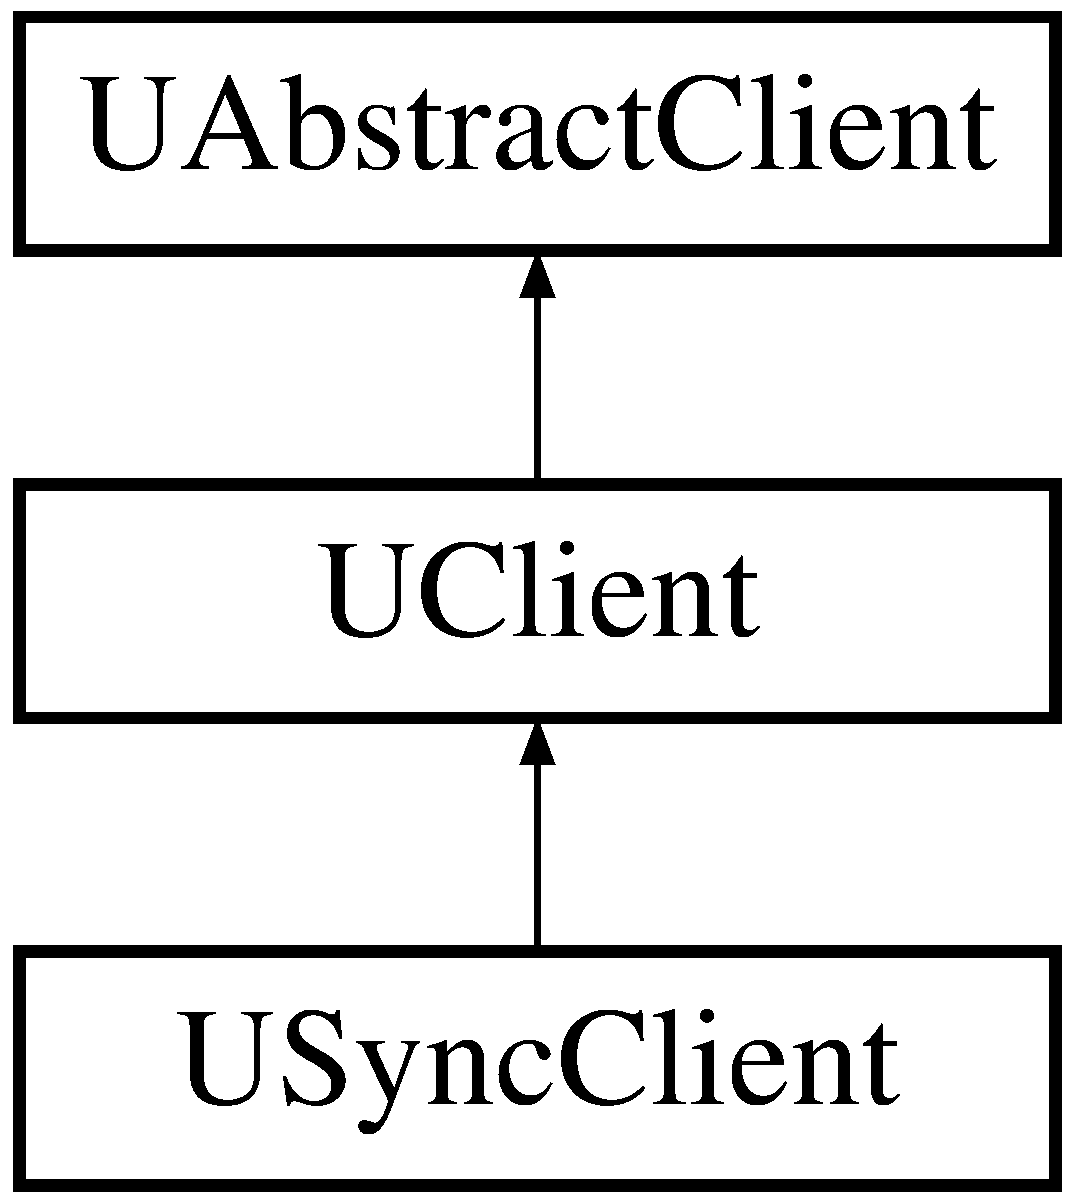
\includegraphics[height=3cm]{classUSyncClient}
\end{center}
\end{figure}
\subsection*{Public Member Functions}
\begin{CompactItemize}
\item 
{\bf USync\-Client} (const char $\ast$\_\-host, int \_\-port={\bf URBI\_\-PORT}, int \_\-buflen={\bf URBI\_\-BUFLEN})\label{classUSyncClient_a0}

\item 
int {\bf sync\-Send} (const void $\ast$buffer, int length)\label{classUSyncClient_a1}

\begin{CompactList}\small\item\em Send given buffer without copying it. \item\end{CompactList}\item 
int {\bf sync\-Get\-Image} (const char $\ast$camera\-Device, void $\ast$buffer, int \&buffersize, int format, int transmit\-Format, int \&width, int \&height)\label{classUSyncClient_a2}

\begin{CompactList}\small\item\em Get an image in a synchronous way. Returns 1 on success, 0 on failure. \item\end{CompactList}\item 
int {\bf sync\-Get\-Device} (const char $\ast$device, double \&val)\label{classUSyncClient_a3}

\begin{CompactList}\small\item\em Get the value of a device in a synchronous way. Returns 1 on success, 0 on failure. \item\end{CompactList}\item 
int {\bf sync\-Get\-Result} (const char $\ast$command, double \&val)\label{classUSyncClient_a4}

\begin{CompactList}\small\item\em Execute an URBI command, return the resulting double value. Returns 1 on success, 0 on failure. \item\end{CompactList}\item 
int {\bf sync\-Get\-Normalized\-Device} (const char $\ast$device, double \&val)\label{classUSyncClient_a5}

\begin{CompactList}\small\item\em Get the normalized value of a device in a synchronous way. Returns 1 on success, 0 on failure. \item\end{CompactList}\item 
int {\bf sync\-Get\-Device} (const char $\ast$device, const char $\ast$field, double \&val)\label{classUSyncClient_a6}

\begin{CompactList}\small\item\em Get a field of a device in a synchronous way. Returns 1 on success, 0 on failure. \item\end{CompactList}\item 
int {\bf sync\-Get\-Sound} (const char $\ast$device, int duration, {\bf USound} \&sound)\label{classUSyncClient_a7}

\begin{CompactList}\small\item\em Get sound for duration milliseconds in buffer. \item\end{CompactList}\end{CompactItemize}


\subsection{Detailed Description}
{\bf UClient}{\rm (p.\,\pageref{classUClient})} linux implementation with support for synchronous functions. 

These functions differs from the {\bf UClient}{\rm (p.\,\pageref{classUClient})} interface in that they are synchronous. One must seriously ponder the fact that they are not easily portable before using them. 



Definition at line 38 of file usyncclient.h.

The documentation for this class was generated from the following files:\begin{CompactItemize}
\item 
{\bf usyncclient.h}\item 
usyncclient.cpp\end{CompactItemize}
